\documentclass{article}

\usepackage{float}
\usepackage{amsmath}
\usepackage{amsfonts}
\usepackage{amssymb}
\usepackage{graphicx}
\usepackage[margin=1in]{geometry}

\usepackage[backend=biber, style=alphabetic, sorting=ynt]{biblatex}

\title{Week 7 - Homework 4}
\author{Artur Topal, S5942128}
\date{\today}

\begin{document}

\maketitle

\begin{center}
  \textbf{TA}: Hanna, grp\_356739\_6
\end{center}

\pagebreak

\section{ Problem H1 } 
A vector field $\mathbf{F}$ is conservative if and only if $\nabla \times \mathbf{F} = \vec{0}$. Verify if that is the case for

\begin{equation}
  \mathbf{F} = (2x + y)\hat{i} + (z\cos(yz) + x)\hat{j} + y\cos(yz)\hat{k}   
\end{equation}

\begin{equation*}
  \nabla \times \mathbf{F} = \begin{vmatrix}
\hat{i} & \hat{j} & \hat{k}\\
\partial_x & \partial_y & \partial_z \\
2x+y & z\cos(yz)+x & y\cos(yz)
  \end{vmatrix} =
\end{equation*}

\begin{equation*}
  = \hat{i} \left(
    \frac{\partial}{\partial y} (y\cos(yz)) -  \frac{\partial}{\partial z} (z\cos(yz)+x)
    \right) - \hat{j} \left(
    \frac{\partial}{\partial x} (y\cos(yz)) -  \frac{\partial}{\partial z} (2x+y)
    \right) + \hat{k} \left(
    \frac{\partial}{\partial x} (z\cos(yz)+x) -  \frac{\partial}{\partial y} (2x+y)
    \right)
\end{equation*}

\begin{equation*}
  = \hat{i} \left( \left[ \cos(yz) - zy\sin(yz) \right] - \left[ \cos(yz) - zy\sin(yz) \right] \right)
  - \hat{j} \left( 0 - 0  \right)
  + \hat{k} \left( 1 - 1  \right) = \vec{0}
\end{equation*}

Since $\mathbf{F}$ is conservative, there exists a function $f(x, y, z) \in C^1$ such that $\mathbf{F} = \nabla f$. Thus we get the following set of equations:

\begin{equation} \label{eq:set}
  \begin{pmatrix}
    2x + y \\ z\cos(yz) + x \\ y\cos(yz)
  \end{pmatrix} = \begin{pmatrix}
    \frac{\partial f}{\partial x} & \frac{\partial f}{\partial y} &  \frac{\partial f}{\partial z} 
  \end{pmatrix}^T
\end{equation}

Integrate the first equation,
\begin{equation} \label{eq:f1}
  f(x, y, z) = \int (2x + y) dx = x^2 + yx + h(y, z)  
\end{equation}

Differentiate eq.~\eqref{eq:f1} with respect to $y$.
\begin{equation} \label{eq:h}
  \frac{\partial f}{\partial y} = x + \frac{\partial h(y,z)}{\partial y}
\end{equation}

Compare eq.~\eqref{eq:h} and eq.~\eqref{eq:set}:
\begin{equation*}
  \frac{\partial f}{\partial y} = x + \frac{\partial h(y,z)}{\partial y} = z\cos(yz) + x \Rightarrow h(y, z) = \int z\cos(yz) dy = \sin(yz) + g(z)
\end{equation*}

Substitute $h(y, z)$ back into eq.~\eqref{eq:f1}
\begin{equation} \label{eq:f2}
  f(x, y, z) = x^2 + yx + \sin(yz) + g(z)
\end{equation}

Differentiate eq.~\eqref{eq:f2} with respect to $z$, and compare with eq.~\eqref{eq:set} to find $g(z)$
\begin{equation*}
  \frac{\partial f}{\partial z} = y\cos(yz) + \frac{dg}{dz} \Rightarrow \frac{\partial f}{\partial z} = y\cos(yz) + \frac{dg}{dz} = y\cos(yz)
\end{equation*}

\begin{equation*}
  \Rightarrow \frac{dg}{dz} = 0 \Rightarrow g(z) = K = const
\end{equation*}

Therefore,
\begin{equation*}
  f(x, y, z) = x^2 + yx + \sin(yz) + K
\end{equation*}

\section{Problem H2}

\subsection{a}
Surface $S$ is a hollow cylinder of radius $1$ extended from $z = 0$ to $z = 1$, and, from $z = 1$ to $z = 9$, it is a hollow cone at $45$ degrees. The Stoke's boundary is composed out of two boundaries $\partial S_1$\footnote{That is, a circle $x^2 + y^2 = 81, z=9$.} and $\partial S_2$\footnote{That is, a circle $x^2 + y^2 = 1, z=0$}. This is because of the (slightly informal) definition of Stoke's boundary [1] and because the specified surface is hollow.

\begin{figure}[H]
  \centering
  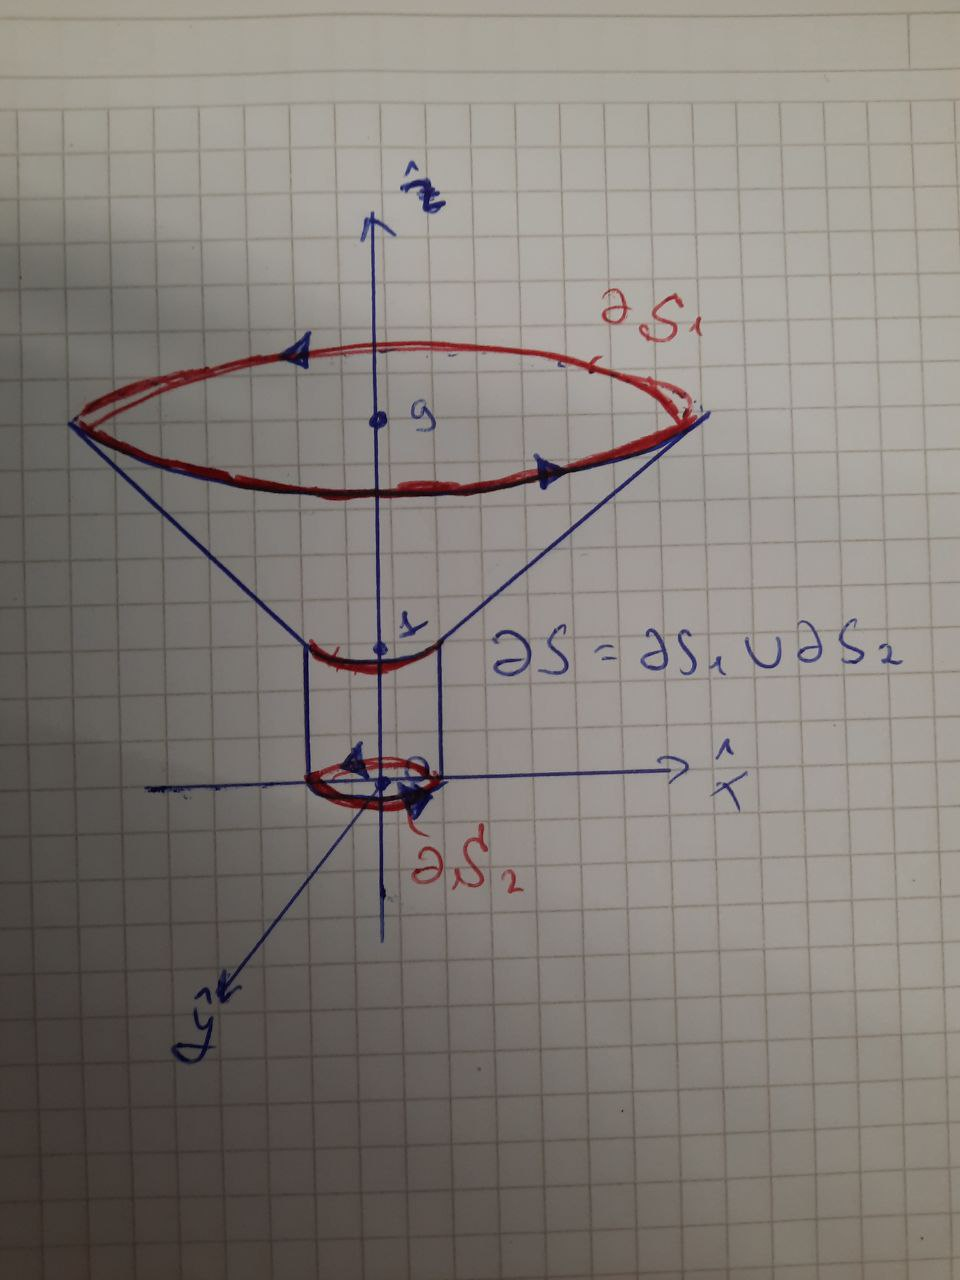
\includegraphics[width=0.3\textwidth]{calculus/W7/img/S}
  \caption{Surface S and its boundary}
  \label{fig:s}
\end{figure}

\subsection{b}
See orientation on Figure \ref{fig:s}. To find unit normal vectors to $S$, notice that $S$ is a piecewise smooth surface. Thus, $S = S_1 + S_2$ where $S_1$ is the cylinder and $S_2$ is the cone. Parametrize $S_1$ and $S_2$
\begin{equation*}
  S_1: \mathbf{r(u, v)} = \begin{pmatrix} \cos u \\ \sin u \\ v  \end{pmatrix}, D = \left\{ (u, v) \subset \mathbb{R} | u \in \left[ 0 ; 2\pi \right], v \in \left[ 0; 1 \right]  \right\}
\end{equation*}

\begin{equation*}
  S_2: \mathbf{r(u, v)} = \begin{pmatrix} v\cos u \\ v\sin u \\ v  \end{pmatrix}, D = \left\{ (u, v) \subset \mathbb{R} | u \in \left[ 0 ; 2\pi \right], v \in \left[ 1; 9 \right]  \right\}
\end{equation*}

Then, unit normal vectors are computed for each surface using $\hat{n} = \frac{\mathbf{r_u} \times \mathbf{r_v}}{|| \mathbf{r_u} \times \mathbf{r_v} ||}$. For $S_1$, $\mathbf{r_u} = \begin{pmatrix} -\sin u \\ \cos u \\ 0  \end{pmatrix}$ and $\mathbf{r_v} = \begin{pmatrix} 0 \\ 0 \\ 1  \end{pmatrix}$. Therefore, the cross product is $\begin{vmatrix} \hat{i} & \hat{j} & \hat{k} \\ -\sin u & \cos u & 0 \\ 0 & 0 & 1 \end{vmatrix} = \begin{pmatrix} \cos u & \sin u & 0  \end{pmatrix}$. Therefore,
\begin{equation*}
  \hat{n_1} = \frac{\begin{pmatrix} \cos u & \sin u & 0  \end{pmatrix}}{|| \begin{pmatrix} \cos u & \sin u & 0  \end{pmatrix} ||} = \frac{\begin{pmatrix} \cos u & \sin u & 0  \end{pmatrix}}{\sqrt{\cos^2 u + \sin^2 u + 0^2}} = \begin{pmatrix} \cos u \\ \sin u \\ 0  \end{pmatrix}
\end{equation*}

Similarly, for $S_2$ surface, $\mathbf{r_u} = \begin{pmatrix} -v\sin u \\ v\cos u \\ 0 \end{pmatrix}$ and $\mathbf{r_v} = \begin{pmatrix} \cos u \\ \sin u \\ 1 \end{pmatrix}$. The cross product is
\begin{equation*}
  \mathbf{r_u} \times \mathbf{r_v} = 
  \begin{vmatrix}
    \hat{i} & \hat{j} & \hat{k} \\
    -v\sin u & v\cos u & 0 \\
    \cos u & \sin u & 1
  \end{vmatrix} =
  \begin{pmatrix}
    v\cos u \\ v\sin u \\ -v \sin^2 u - v\cos^2 u
  \end{pmatrix} =
  \begin{pmatrix}
    v\cos u \\ v\sin u \\ -v
  \end{pmatrix}
\end{equation*}
\begin{equation*}
  ||\mathbf{r_u} \times \mathbf{r_v}|| = \sqrt{v^2\cos^2 u + v^2\sin^2 u + (-v)^2} = v\sqrt{2}
\end{equation*}
Thus, the unit normal vector to $S_2$ is
\begin{equation*}
  \hat{n_2} = \frac{1}{v\sqrt{2}} \begin{pmatrix}
    v\cos u \\ v\sin u \\ -v
  \end{pmatrix} = \begin{pmatrix}
    \sqrt{2}/2\cos u \\ \sqrt{2}/2\sin u \\ -\sqrt{2}/2
  \end{pmatrix}
\end{equation*}

\subsection{c}
Given: $\mathbf{V} = -y\hat{i} + x\hat{j} + z\hat{k}$. Since surface $S$ is not closed, the flux can be computed directly.
\begin{equation*}
  \iint_{S} \mathbf{V} \cdot d\mathbf{S} = \iint_{S_1} \mathbf{V} \cdot d\mathbf{S} + \iint_{S_2} \mathbf{V} \cdot d\mathbf{S}
\end{equation*}

\begin{equation*}
  S_1: \iint_{S_1} \mathbf{V} \cdot d\mathbf{S} = \int_{u=0}^{2\pi} \int_{v=0}^{1} \mathbf{V(r(u, v))} \cdot \begin{pmatrix} \cos u \\ \sin u \\ 1 \end{pmatrix} dvdu = \int_{u=0}^{2\pi} \int_{v=0}^{1} \begin{pmatrix} -\sin u \\ \cos u \\ v \end{pmatrix} \cdot \begin{pmatrix} \cos u \\ \sin u \\ 1 \end{pmatrix} dvdu
\end{equation*}
\begin{equation*}
   = \int_{u=0}^{2\pi} \int_{v=0}^{1} -\sin u \cos u + \cos u \sin u + v  dvdu = \int_{u=0}^{2\pi} \int_{v=0}^{1} vdvdu = \int_{u=0}^{2\pi} \left[\frac{v^2}{2} \right]_{0}^{1} du = \frac{1}{2} \int_{u=0}^{2\pi} du = \frac{2\pi - 0}{2}
 \end{equation*}
 \begin{equation*}
   \Rightarrow \iint_{S_1} \mathbf{V} \cdot d\mathbf{S} = \pi
 \end{equation*}
\begin{equation*}
  S_2: \iint_{S_2} \mathbf{V} \cdot d\mathbf{S} = \int_{u=0}^{2\pi} \int_{v=1}^{9} \mathbf{V(r(u, v))} \cdot \hat{n_2} dvdu = \int_{u=0}^{2\pi} \int_{v=1}^{9} \begin{pmatrix} -v\sin u \\ v\cos u \\ v \end{pmatrix} \cdot \begin{pmatrix} \sqrt{2}/2\cos u \\ \sqrt{2}/2\sin u \\ -\sqrt{2}/2 \end{pmatrix} dvdu
\end{equation*}
\begin{equation*}
  = \int_{u=0}^{2\pi} \int_{v=1}^{9} \left( -v\sin u \frac{\sqrt{2}}{2}\cos u + v\cos u \frac{\sqrt{2}}{2} \sin u - \frac{\sqrt{2}}{2}v \right)  dvdu = -\frac{\sqrt{2}}{2} \int_{u=0}^{2\pi} \int_{v=1}^{9}  v dvdu = -\frac{\sqrt{2}}{2} \int_{u=0}^{2\pi} \left[\frac{v^2}{2} \right]_{1}^{9} du
\end{equation*}
\begin{equation*}
  -\frac{\sqrt{2} \cdot 40}{2} \int_{0}^{2\pi} du  = -\sqrt{2} \cdot 20 \cdot 2\pi = -40\pi\sqrt{2} \Rightarrow \iint_{S_2} \mathbf{V} \cdot d\mathbf{S} = -40\pi\sqrt{2}
\end{equation*}

The total flux is thus $\pi - 40\pi\sqrt{2}$

\textbf{Answer}: $\iint_S \mathbf{V} \cdot d\mathbf{S} =  \pi(1 - 40\sqrt{2})$
\begin{thebibliography}{99}

\bibitem{boundary}
{The Stoke's boundary}, {Toronto University, Mathematics Department}, Available: \url{https://www.math.utoronto.ca/courses/mat237y1/20189/notes/Chapter5/S5.6.html#sect-5.6.1}, Accessed: 07/01/2025.
  
\end{thebibliography}


\end{document}
